\documentclass[12pt]{aghdpl}
% \documentclass[en,11pt]{aghdpl}  % praca w języku angielskim

% Lista wszystkich języków stanowiących języki pozycji bibliograficznych 
%użytych w pracy.
% (Zgodnie z zasadami tworzenia bibliografii każda pozycja powinna zostać 
% utworzona zgodnie z zasadami języka, w którym dana publikacja została napisana.)
\usepackage[english,polish]{babel}

% Pakiet do wielkości czcionki
%\usepackage[12pt]{extsizes}

% Użyj polskiego łamania wyrazów (zamiast domyślnego angielskiego).
\usepackage{polski}

\usepackage[utf8]{inputenc}

% dodatkowe pakiety

\usepackage{mathtools}
\usepackage{amsfonts}
\usepackage{amsmath}
\usepackage{amsthm}

% --- < hiperlacza > ---
\usepackage{hyperref}
\hypersetup{
    colorlinks,
    citecolor=black,
    filecolor=black,
    linkcolor=black,
    urlcolor=black
}

% --- < bibliografia > ---

\usepackage[
style=numeric,
sorting=none,
%
% Zastosuj styl wpisu bibliograficznego właściwy językowi publikacji.
language=autobib,
autolang=other,
% Zapisuj datę dostępu do strony WWW w formacie RRRR-MM-DD.
urldate=iso8601,
% Nie dodawaj numerów stron, na których występuje cytowanie.
backref=false,
% Podawaj ISBN.
isbn=true,
% Nie podawaj URL-i, o ile nie jest to konieczne.
url=false,
%
% Ustawienia związane z polskimi normami dla bibliografii.
maxbibnames=3,
% Jeżeli używamy BibTeXa:
backend=bibtex
]{biblatex}

\usepackage{csquotes}
% Ponieważ `csquotes` nie posiada polskiego stylu, można skorzystać z mocno 
% zbliżonego stylu chorwackiego.
\DeclareQuoteAlias{croatian}{polish}

\addbibresource{bibliografia.bib}

% Nie wyświetlaj wybranych pól.
%\AtEveryBibitem{\clearfield{note}}


% ------------------------
% --- < listingi > ---

% Użyj czcionki kroju Courier.
\usepackage{courier}

\usepackage{listings}
\lstloadlanguages{TeX}

\lstset{
	literate={ą}{{\k{a}}}1
           {ć}{{\'c}}1
           {ę}{{\k{e}}}1
           {ó}{{\'o}}1
           {ń}{{\'n}}1
           {ł}{{\l{}}}1
           {ś}{{\'s}}1
           {ź}{{\'z}}1
           {ż}{{\.z}}1
           {Ą}{{\k{A}}}1
           {Ć}{{\'C}}1
           {Ę}{{\k{E}}}1
           {Ó}{{\'O}}1
           {Ń}{{\'N}}1
           {Ł}{{\L{}}}1
           {Ś}{{\'S}}1
           {Ź}{{\'Z}}1
           {Ż}{{\.Z}}1,
	basicstyle=\footnotesize\ttfamily,
}

% ------------------------

\AtBeginDocument{
	\renewcommand{\tablename}{Tabela}
	\renewcommand{\figurename}{Rys.}
}

% ------------------------
% --- < tabele > ---

\usepackage{array}
\usepackage{tabularx}
\usepackage{multirow}
\usepackage{booktabs}
\usepackage{makecell}
\usepackage[flushleft]{threeparttable}
\usepackage{float}

% defines the X column to use m (\parbox[c]) instead of p (`parbox[t]`)
\newcolumntype{C}[1]{>{\hsize=#1\hsize\centering\arraybackslash}X}


%---------------------------------------------------------------------------

\author{Bartłomiej Styczeń}
\shortauthor{B. Styczeń}

%\titlePL{Przygotowanie bardzo długiej i pasjonującej pracy dyplomowej 
% w~systemie~\LaTeX}
%\titleEN{Preparation of a very long and fascinating bachelor or master 
%thesis in \LaTeX}

\titlePL{Kognitywny system eksploracji środowiska przez inteligentnego agenta 
z wykorzystaniem uczenia motywowanego.}
\titleEN{Cognitive system of environment exploration by an intelligent agent 
using motivated learning}


\shorttitlePL{Kognitywny system ekspolarcji środowiska z wykorzystaniem 
uczenia motywowanego} % skrócona wersja tytułu jeśli jest bardzo długi
\shorttitleEN{Cognitive system of environment exploration using 
motivated learning}

\thesistype{Praca dyplomowa magisterska}
%\thesistype{Master of Science Thesis}

\supervisor{dr hab. Adrian Horzyk}
%\supervisor{Marcin Szpyrka PhD, DSc}

\degreeprogramme{Automatyka i robotyka}
%\degreeprogramme{Computer Science}

\date{2015}

\department{Katedra Automatyki i Robotyki}
%\department{Department of Applied Computer Science}

\faculty{Wydział Elektrotechniki, Automatyki,\protect\\[-1mm] Informatyki 
i Inżynierii Biomedycznej}
%\faculty{Faculty of Electrical Engineering, Automatics, Computer Science 
% and Biomedical Engineering}

\acknowledgements{Serdecznie dziękuję \dots tu ciąg dalszych podziękowań 
np. dla promotora, żony, sąsiada itp.}


\setlength{\cftsecnumwidth}{10mm}

%---------------------------------------------------------------------------
\setcounter{secnumdepth}{4}
\brokenpenalty=10000\relax

\begin{document}

\titlepages

% Ponowne zdefiniowanie stylu `plain`, aby usunąć numer strony z pierwszej strony spisu treści i poszczególnych rozdziałów.
\fancypagestyle{plain}
{
	% Usuń nagłówek i stopkę
	\fancyhf{}
	% Usuń linie.
	\renewcommand{\headrulewidth}{0pt}
	\renewcommand{\footrulewidth}{0pt}
}

\setcounter{tocdepth}{2}
\tableofcontents
\clearpage

\chapter{Wprowadzenie}
\label{cha:wprowadzenie}

Ta praca jest o~uczeniu motywowanym przy eksploracji środowiska przez agenta, 
który w~przypadku tej pracy dyplomowej będzie wykonywana na robocie mobilnym. 
Zastosowane zostanie środowisko symulacyjne umożliwiające sterowanie takim 
robotem, odczytywanie różnych parametrów środowiska otaczającego agenta, 
także tych, których sensory robota, np. kamera, czujniki odległości, nie 
umożliwiają do odczytania.

%---------------------------------------------------------------------------

\section{Cele pracy}
\label{sec:cele_pracy}

Celem poniższej pracy jest zastosowanie uczenia motywowanego do eksploracji 
nieznanego środowiska przez agenta (robota mobilnego) i~porównanie osiągnięć 
takiego agenta w~porównaniu z~podobnym agentem wykorzystującym algorytmy uczenia 
ze wzmocnieniem, np. przy jednoczesnej lokalizacji i~mapowaniu SLAM (ang. 
\textit{simultaneous localization and mapping}).

%---------------------------------------------------------------------------

\section{Zawartość pracy}
\label{sec:zawartosc_pracy}

Ta część będzie napisana jak cała reszta pracy zostanie ukończona\dots

\chapter{Uczenie motywowane}
\label{cha:rozdzial2}

Człowiek od momentu, kiedy jest wstanie poznawać swoje środowisko, w którym się 
znajduje ma ochotę eksplorować na swoje możliwości. Małe dzieci, które nie 
umieją jeszcze chodzić albo raczkować, mogą tworzyć skojarzenia pomiędzy 
różnymi czynnikami. Jednym z przykładów może być nawet karmienie takiego 
dziecka małą butelką i poprzez umożliwianie mu trzymanie tej butelki 
samodzielnie, małe dziecko będzie w stanie po pewnym czasie utworzyć 
skojarzenie, że jeżeli będzie trzymało mocno butelkę i w odpowiedniej pozycji, 
to będzie mogło zjeść w razie głodu.

Eksploracja środowiska i swobodne poznawanie go, umożliwia tworzenie połączeń 
asocjacji pomiędzy pewnymi obserwacjami, akcjami jakie wykonaliśmy na nich oraz 
rezultatów jakie zostały otrzymanie w wyniku takich a nie innych akcji. Innym 
przykładem u małego człowieka jest to, że niepilnowane młode dziecko może 
dotknąć czegoś gorącego i się oparzyć, mimo, że rodzice zabronili tego. Dopiero 
poczucie fizycznego bólu sprawi, że dziecko będzie dobrze pamiętało, żeby 
więcej tego nie robić. Dlatego też człowiek często uczy się na własnych błędach 
najlepiej, kiedy sam czegoś doświadczy.

Kluczowe dla uczenia motywowanego (ang. \textit{motivated learning}) jest 
pojęcie motywacji w ucieleśnionej inteligencji (ang. \textit{motivation in 
embodied intelligence}). Inteligencja ucieleśniona jest obliczeniowym 
podejściem do projektowania i rozumienia inteligentnego zachowania u 
ucieleśnionych agentów poprzez wzięcie pod uwagę ścisłego powiązania między 
agentem, a jego otoczeniem. Należy brać pod uwagę jego ograniczenia tj. 
ograniczenia własnego ciała (ograniczenia mechaniczne i/lub elektryczne 
robota), systemu percepcyjnego (systemy wizyjne i ich sprzętowe ograniczenia) 
oraz motoryczne. Jedną z najbardziej wpływowych postaci w procesie 
projektowania ucieleśnionej inteligencji jako metodologii był Rodney Brooks. 
Zasugerował on tworzenie inteligentnych maszyn poprzez interakcję ze 
środowiskiem napędzane przez percepcję i akcję niż przez konkretne 
wyspecjalizowany algorytm.

W dzisiejszy czasach badania w zakresie sztucznej inteligencji są kojarzone z 
wyspecjalizowanym rozwiązywaniem problemów tj. reprezentacja wiedzy, 
zrozumienie języka naturalnego czy oglądanej sceny czy odpowiadanie na pytania. 
Wszystkie te zagadnienia są bardzo ciekawe i sprawiają, że wiele problemów 
zostaje rozwiązywane przez komputery. Jednak nie ma w nich systemu, który spaja 
wszystkie te zagadnienia w jeden system, który mógłby być określaną "silną 
inteligencją".

\section{Definicje związane z projektowaniem ucieleśnionej inteligencji}

W celu projektowania maszyn ucieleśnionej inteligencji zostały zdefiniowane 
pewne zasady i założenia. Pierwszym z nich było to, że agent rozwija się w 
zmieniającym środowisku, które może manipulować i postrzegać korzystając z 
dostępnych sensorów. Nie istnieje potrzeba tworzenia modelu środowiska, 
ponieważ ono się może zmieniać. 

Dodatkowe reguły projektowania zostały zawarte w \cite{pfeifer_ei}:
\begin{enumerate}
	\item Reguła taniego projektu i nadmiarowości -- projekt maszyny powinien 
	być prosty i jego projekt sprawiał, że funkcjonalności podzespołów nachodzą 
	na siebie pozwalając na działanie maszyny w razie awarii jakiegoś 
	podzespołu.
	\item Reguła równoległych, luźno związanych procesów -- ta reguła wymusza 
	na maszynie to, że inteligencja pojawia się przez interakcję 
	niskopoziomowych procesów np. sterowania ramionami ze środowiskiem.
	\item Reguła wartości -- reguła ta może wymuszać, aby maszyna robiła, to co 
	jest dobre dla niej. Umożliwia ona sugerowanie maszynie, co powinna zrobić 
	w danej sytuacji (agenty uczenia ze wzmocnieniem uczą się korzystając m.in. 
	z tej reguły)
\end{enumerate}
		
\section{Inteligencja}
Do dzisiaj nie ma dokładnej definicji inteligencji. Jest wiele interpretacji, a 
jednocześnie należy mieć na uwadze, aby nie mylić inteligencji ze złożonym 
zachowaniem. To bardzo ważne, ponieważ możemy wziąć pewien algorytm, np. 
szukania najkrótszej ścieżki w grafie, która ogółem jest złożonym problemem, 
który składa się ze skończonej liczby kroków. Zdecydowanie nie można 
stwierdzić, że ten algorytm jest inteligenty. To tylko pewien zbiór prostych 
czynności, które rozwiązują konkretny problem i użyte do czegoś innego (można 
tak nazwać zmieniające się środowisko), na pewno nie da dobrych rezultatów.

Opisy inteligencji skupiają się na opisie właściwości umysły, niż samym umyśle. 
W swojej pracy \cite{stewart_93} John Stewart zdefiniował systemy kognitywne 
jako:

\textbf{Definicja:} System jest kognitywny wtedy i tylko wtedy, gdy wejścia z 
sensorów powodują akcje w konkretny sposób, tak aby spełnić wymagania do 
przeżycia w środowisku. 


\textbf{Definicja:} Uczeleśniona inteligencja (ang. \textit{embodied 
intelligence} EI) jest zdefiniowana jako mechanizm, który uczy się jak 
przetrwać we wrogim środowisku (wrogie można także określić jako zmieniające 
się).

Ta druga definicja odnosi się do wszystkich form ucieleśnionej inteligencji: 
biologicznej, mechanicznej czy wirtualnych agentów. Wynika z tego, że agent EI 
wchodzi w interakcje ze środowiskiem i postrzega wprowadzone zmiany poprzez 
sensory. Agent musi się nauczyć jak przetrwać w środowisku. Natomiast wrogość 
środowiska może być określana na różne sposoby. Może to być jego ciągła 
zmienność, czy mała dostępność surowców potrzebnych agentowi przetrwania. Ważne 
jest to, że ta wrogość jest stała. Przykładowo, poziom naładowania baterii jest 
stałych zagrożeniem dla agenta. Jeżeli poziom naładowania będzie się 
zmniejszał, to dyskomfort wywoływany przez sensor odpowiedzialny za pomiar 
baterii będzie rósł.

Kolejnym ważnym elementem definicji ucieleśnionej inteligencji jest aspekt 
uczenia. Jeżeli agent wie jak przetrwać we wrogim środowisku, ale nie wie jak 
się nauczyć nowych umiejętności, nie jest inteligentny. Przykładowo, algorytm, 
która zajmuje się sterowaniem jakiegoś procesu technologicznego nie jest 
inteligentny, ponieważ nie będzie w stanie nauczyć się sterować samochodem. W 
zamierzeniu jego zadaniem było regulowanie wartości zadanej konkretnego procesu 
technologicznego.

Należy zwrócić uwagę, że EI odróżnia wiedzę od inteligencji. Wiedza może być w 
pewien sposób zintegrowana z agentem w trakcie jego projektowania, np. jako 
zbiór pewnych reguł zachowania. Natomiast inteligencja sprawia, że ta wiedza 
może być użyta do tworzenia nowych umiejętności i zarządzania nimi w sposób 
zorganizowany i koherentny.

\section{Projektowanie ucieleśnionej inteligencji}

Uczenie jest aktywnym procesem. Informacje o otoczeniu EI zdobywa poprzez 
koordynację pary sensor -- motor. Uczenie się, które akcje są pożądane, a które 
nie, sprawiają, że agent uczący jest lepiej przystosowany do wrogiego 
środowiska. Można odróżnić co najmniej dwa sposoby na adaptowanie do zmiennego 
środowiska \cite{motivation_in_ei}:

\begin{enumerate}
	\item ewolucyjne -- naturalna selekcja agentów (gatunków zwierząt), które 
	są najlepiej przystosowane lub rozwój nowych umiejętności np. pocenie się, 
	aby utrzymać odpowiednią temperaturę,
	
	\item kognitywne -- poprzez uczenie, używając pamięci i asocjacji, stosując 
	rozpoznawanie schematów, budowanie reprezentacji i implementowanie celów.
\end{enumerate}

Schematy na wielu poziomach abstrakcji są uczone i zapamiętywane przez agenta. 
Pewne abstrakcyjne reprezentacje są budowane aby reprezentować akcje i 
umiejętności. Cała struktura wzorów i relacji pomiędzy nimi jest reprezentowana 
w pewnej postaci w pamięci, która jest asocjacyjna i epizodyczna. Ten system 
jest rozproszony, nadmiarowy i równoległy a dodatkowo krótko i długoterminowy. 
Cały ten system łączy się ze sobą i wchodzi w interakcję w czasie rzeczywistym.

Krytycznym aspektem rozwoju umysłu człowieka jest samoorganizacja. Dzięki niej 
neurony mogą szybko tworzyć nowe reprezentacje zapamiętanych schematów, uczyć 
się jak wchodzić w interakcję z otoczeniem oraz budować oczekiwania związane z 
przyszłymi wydarzeniami, czyli umiejętność prognozowania przyszłych wydarzeń na 
podstawie aktualnego stanu oraz tego, co stało się w przeszłości.

Agent uczenia motywowanego dzieli wspólne właściwości ze specjalnym typem 
agenta racjonalnego (ang. \textit{rational software agent}) znanego jako agenta 
przekonań -- pragnień -- intecji (ang. \textit{belief -- desire -- intention}). 
To pewien z modeli tworzenia oprogramowania, który umożliwia rozdzielenie 
funkcjonalności od siebie. Ten model skupia się na planowaniu i sposobie 
wykonania pewnych zadań. Cechy wspólne z agentem uczenia motywowanego to 
tworzenie reprezentacji poznanego środowiska, pragnienia to motywacje dla 
agenta motywowanego. Różnicą jest sposób implementacji reprezentacji wiedzy. 
Dla agenta uczenia motywowanego nie ma konkretnego sposobu implementacji, 
ponieważ widza ta jest reprezentowana przez struktury sieci neuronowych a tym 
samym wszelkie plany, co do wykonywanych akcji muszą być pochodzą z aktywacji 
neuronów w sieci neuronowej.


\section{Ból jako motywacja}

Zadaniem każdej maszyny jest wykonywanie pewnych z góry określonych zadań. 
Pytaniem jest, co może być motywujące, aby dana maszyna/program wykonywały go w 
sposób perfekcyjny. Dla pewnych grup algorytmów można zdefiniować z góry 
określoną funkcję kosztu, którą w sposób iteracyjny usprawnia działanie danego 
algorytmu. Jednakże takie podejście daje bardzo mało możliwości do 
generalizowania zdobytych umiejętności na nowe potrzeby, np. zmiennego 
środowiska.

Aby odpowiedzieć na pytanie, co może motywować maszyny do ulepszania swoich 
możliwości w sposób bardziej zgeneralizowany, można zastanowić się, co motywuje 
ludzi do rozwijania swoich umiejętności. Próbą odpowiedzi na to pytanie podjął 
się psycholog Csíkszentmihályi w książce opisującej teorię przepływu 
\cite{csikszentmihalyi1996creativity}. W tej teorii opisano, że ludzie 
otrzymują wewnętrzne nagrody za wszelkie aktywności, które są trochę ponad ich 
aktualny poziom rozwoju. 

Starzyk w pracy \cite{motivation_in_ei} sugeruje, że to wrogość środowiska, 
które jest ujęte w definicji agenta ucieleśnionej inteligencji (EI) jest 
najbardziej efektywnym czynnikiem motywującym do uczenia. Ma to odniesienie do 
ludzkiego sposobu uczenia. Podstawowym bólem może być ciekawość. To ona 
sprawia, że chcemy poznawać nowe rzeczy. Dla małego dziecka taka ciekawość może 
wywołać ból fizyczny, kiedy z ciekawości oparzy się dotykając czegoś gorącego. 
Ale ten ból sprawi, że w przyszłości będzie wiedziało jak postępować, aby nie 
zwiększać tego bólu.

Według Starzyka bóle prymitywne są bezpośrednio związane z bodźcami odbieranymi 
przez sensory maszyny. Natomiast definiuje on bóle abstrakcyjne (ang. 
\textit{abstract pains}). Pojawiają się one, kiedy agent nie jest w stanie 
wykonać akcji, która zmniejszy wartość bólu prymitywnego. W ten sposób mogą się 
tworzyć struktury grafowe opisujące relacje pomiędzy różnymi bólami. Co ważne, 
bóle abstrakcyjne nie są stymulowane przez sensor wartości fizycznej, np. niski 
poziom naładowania baterii dla robota.  
\ref{fig:abstractpainscreation}.

\begin{figure}[H]
	\centering
	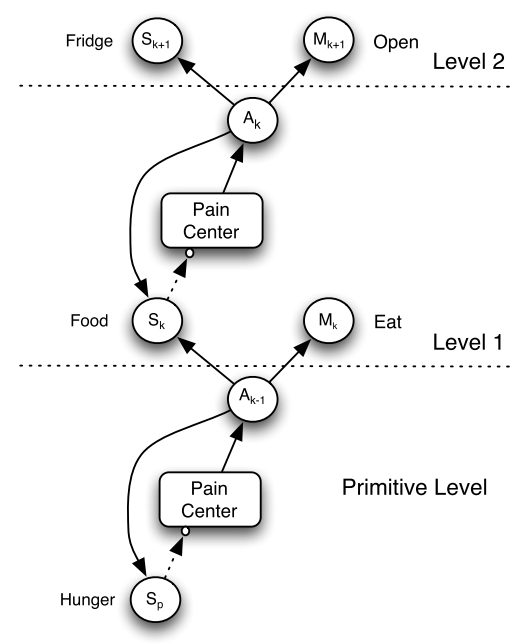
\includegraphics[width=0.5\linewidth]{rozdzial2/images/abstract_pains_creation}
	\caption{Tworzenie sygnałów abstrakcyjnych bóli. Źródło: 
	\cite{ml_dev_auto_systems}}
	\label{fig:abstractpainscreation}
\end{figure}

Bóle tworzą hierarchię wszerz i wgłąb, tworząc struktury grafowe. 
W takich strukturach teoretycznie mogą pojawiać się zamknięte ścieżki, np. brak
jedzenia może sprawić, żeby kupić więcej jedzenia, a do tego potrzebne są 
pieniądze, które można zdobyć sprzedając jedzenie. Należy wziąć pod uwagę takie 
sytuacje w procesie tworzenia całej architektury i sposobu uczenia maszyny.

\section{Tworzenie celów w uczeniu motywowanym}

Jednym z podstawowych źródeł tworzenia nowych celów jest wcześniej wspomniany 
ból. Najbardziej prymitywnym bólem u ludzi jest uczucie dyskomfortu, gdy czują 
głód. W maszynach można to odnieść do poziomu naładowania baterii w robocie i 
coraz niższy poziom sprawia, że ból związany z brakiem energii zwiększa się. 
Agent uczenia motywowanego musi się nauczyć jak ten ból zmniejszać, tak jak 
człowiek uczy się zdobywać jedzenie oraz jeść. Mimo, że wszelkie abstrakcyjne 
bóle, które wykształcają się w dalszym rozwoju, to te prymitywne umożliwiają 
realizację kolejnych zadań czy celów.

Dokładny opis algorytmu tworzenia celów został opisany w 
\cite{ml_comp_int}

\textbf{Algorytm tworzenia celów (ang. \textit{goal creation system})}
\begin{enumerate}
    \item Wybierz dominujący ból stosując regułę zwycięzca bierze wszystko 
        (ang. \textit{winner takes all}) spomiędzy konkurujących ośrodków bólu.
        \begin{itemize}
            \item Jeżeli żaden z bóli nie przekracza wcześniej zdefiniowanego 
                progu, czekaj aż któryś z nich przekroczy ten próg.
        \end{itemize}
    \item Jako aktualny cel wybierz zmniejszenie dominującego bólu.
        \begin{itemize}
            \item aktualny cel motywuje agenta do działania.
        \end{itemize}
    \item Wybierz wcześniej nauczoną akcje, która z najwyższym 
          prawdopodobieństwem spełni aktualny cel.
        \begin{itemize}
            \item Jeżeli nie ma żadnego, idź do punktu 6.
        \end{itemize}
    \item Sprawdź czy wybrana czynność może być wykonana w aktualnym środowisku. 
        Jeśli nie, idź do punktu 3.
    \item Wykonaj akcję.
        \begin{itemize}
            \item Jeśli ta akcja \textit{obniżyła} wartość dominującego bólu:
                \begin{enumerate}
                    \item Zwiększ wartości wag zależności pomiędzy aktualnym 
                        bólem a~akcją jaka została wykonana i~zwiększ wartość 
                        wag odpowiadających abstrakcyjnemu bólowi powiązanego 
                        z~tą akcją.
                    \item Idź do punktu 1.
                \end{enumerate}
            \item Jeśli ta akcja \textit{nie obniżyła} wartości dominującego bólu.
                \begin{enumerate}
                    \item Zmniejsz wartości wag zależności pomiędzy aktualnym 
                        bólem a~akcją jaka została wykonana i~zmniejsz wartość 
                        wag odpowiadających abstrakcyjnemu bólowi powiązanego 
                        z~tą akcją.
                    \item Idź do punktu 3.
                \end{enumerate}
        \end{itemize}
    \item Wykonaj eksplorację przestrzeni akcji mającą na celu spełnienie celu.
        \begin{itemize}
            \item Jeśli nowa akcja \textit{zmniejszyła} wartość dominującego bólu.
                \begin{enumerate}
                    \item Zwiększ wartości wag zależności pomiędzy aktualnym 
                        bólem a~akcją jaka została wykonana i~stwórz nowy 
                        abstrakcyjny ból związany z~niemożliwością wykonania 
                        tej akcji.
                    \item Idź do punktu 1.
                \end{enumerate}
            \item Jeśli nowa akcja \textit{nie zmniejszyła} wartości 
                dominującego bólu, idź do punktu 6.
        \end{itemize}
\end{enumerate}

Uczenie motywowane może być zastosowane wspólnie z~uczeniem opartym na 
ciekawości (ang. \textit{curiosity based learning}) -- ciekawość poinformuje 
agenta o~nowych odkryciach, podczas gdy uczenie motywowane skupi się na 
poszukiwaniu konkretnych celów, które nie są podane przez twórcę (tak jak 
w~uczeniu ze wzmocnieniem).

\section{Podstawowy element systemu tworzenia celów}

Mechanizm budowania celów składa się z wielu, prostych elementów nazywanych 
jednostkami tworzenia celów (ang. \textit{goal creation unit}). Składa się on 
głównie z trzech typów neuronów, które wchodzą ze sobą w interakcję. Są to:

\begin{itemize}
	\item neurony odpowiadające za ból (ang. \textit{pain center neurons}),
	\item neurony wzmacniające lub zmniejszające odczucie bólu (ang. 
	\textit{reinforcement neuro-transmitter neurons}),
	\item neurony odpowiadające za motorykę (ang. \textit{neurons in sensory 
	and motor pathway}).
\end{itemize}

Schemat reprezentujący połączenia zawarto na rysunku 
\ref{fig:goalcreationsystemunit}.

\begin{figure}[H]
	\centering
	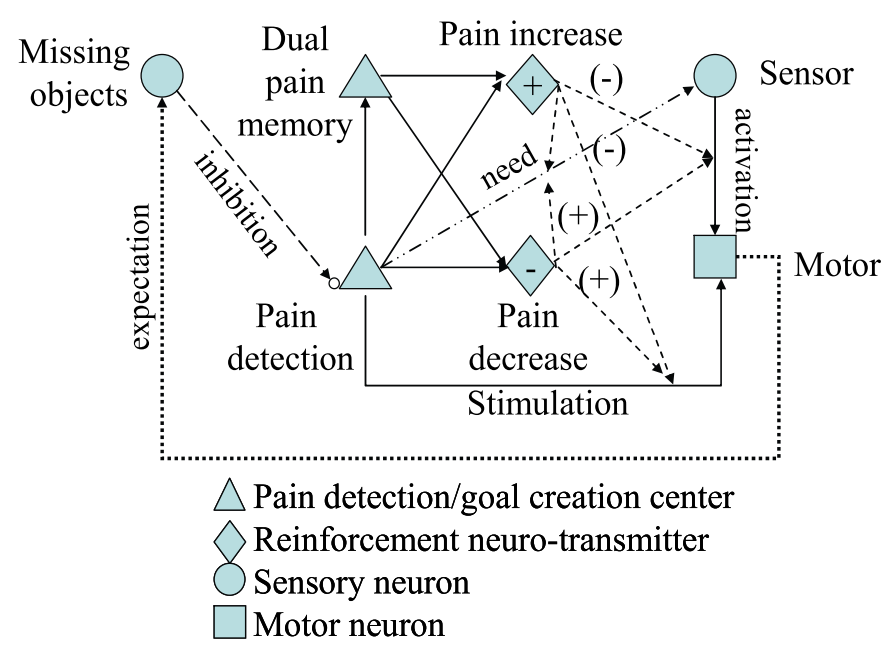
\includegraphics[width=0.7\linewidth]{rozdzial2/images/goal_creation_system_unit}
	\caption{Schemat podstawowego elementu systemu tworzenia celów. Źródło: 
	\cite{motivation_in_ei}.}
	\label{fig:goalcreationsystemunit}
\end{figure}

Neurony odpowiadające za odczuwanie bólu (te po lewej stronie na rysunku 
\ref{fig:goalcreationsystemunit}) są stymulowane przez sygnał reprezentujący 
ból oznaczany przez $I_P$. Reprezentuje on negatywny stymulant, np. ból, 
dyskomfort czy nieprzyjemność. Ponieważ ból istnieje z powodu braku czegoś w 
środowisku (oznaczone na rysunku jako "missing objects"), to neurony 
odpowiedzialne za detekcję bólu aktywują się w momencie wyciszenia neuronu 
odpowiedzialnego za czytanie wartości z otoczenia. Dodana została także pamięć 
wartości bólu z poprzedniego wydarzenia, oznaczone jako $I_{Pd}$. Neurony 
wykorzystują tą wartość do wzmacniania uczucia odczuwania bólu, jeżeli 
zwiększył się on od poprzedniego wydarzenia. Wartość tego wzmocnienia zapisano 
w równaniu \ref{equ:reinforcement_pain}.

\begin{equation}
	\label{equ:reinforcement_pain}
	r = I_P - I_{Pd}
\end{equation}

Ostatnią grupą (po prawej stronie na rysunku \ref{fig:goalcreationsystemunit}) 
są neurony odpowiedzialne za obliczanie wartości akcji jakie ma wykonać robot. 
Na początku centrum detekcji bólu bezpośrednio wpływa na neurony odpowiedzialne 
za wykonywanie akcji, ponieważ wszelkie wagi neuronów $W_{MP}$ są losowo 
zainicjalizowane. W trakcie poznawania środowiska, maszyna dostraja wartości 
tych wag. Dodatkowo, aby pewna akcja była wykonana muszą być dostępne pewne 
obiekty z otoczenia (na rysunku \ref{fig:goalcreationsystemunit} oznaczone jako 
"Sensor" po prawej stronie). Na początku neuron będzie miał powiązania z 
wieloma różnymi obiektami poprzez losowa zainicjalizowane wagi $W_{MS}$.

Po wykonanej akcji, która zmniejszyła albo zwiększyła wartość odczuwanego bólu 
(wykrytego przez drugą grupę neuronów odpowiedzialną za detekcję bólu), 
generowany jest sygnał $r$ (obliczony zgodnie z równaniem 
\ref{equ:reinforcement_pain}). Wykorzystywany jest to wzmocnienia lub 
osłabienia wag $W_{MP}$ i $W_{MS}$ zgodnie z równaniem \ref{equ:weights_update}

\begin{equation}
	\label{equ:weights_update}
	\begin{aligned}
		W_{MP} = W_{MP} + r \cdot \beta ^ n \\
		W_{MS} = W_{MS} + r \cdot \beta ^ n
	\end{aligned}
\end{equation}

gdzie:
\begin{itemize}
	\item $\beta$ -- oznacza współczynnik uczenia, mniejszy od wartości 1,
	\item $n$ -- oznacza jak wiele razy dane połączenie było zmieniane.
\end{itemize}

Dodatkowo neuron odpowiedzialny za reprezentację obiektu, który był użyty do 
zmniejszenia bólu zostanie dodany z wagą $W_{SP}$ w celu połączenia centrum 
detekcji bólu z neuronem sensorycznym. Ten neuron będzie uczony korzystając 
uczenia metodą Hebba.

Z kolei z drugiej strony, obiekt, którego zabrakło i stworzył on ból 
abstrakcyjny, staje się dostępny. Zostaje stworzony neuron reprezentujący 
połączenie neuronu odpowiedzialnego za motorykę z neuronem z brakującym 
obiektem z wagą $W_{SM}$.

Oba wymienione wcześniej połączone będą uczone metodą wzmocnienia. Oznacza to, 
że im mocniejsza zmiana poziomu bólu, tym mocniejsza korekta wartości tych wag. 




\chapter{Uczenie ze wzmocnieniem}
\label{cha:rozdzial3}

Kilka słów o uczeniu ze wzmocnieniem\dots

\chapter{Uczenie motywowane i ze wzmocnieniem -- porównanie}
\label{cha:rozdzial4}

Wyniki eksperymentów zawarte w \cite{ml_comp_int} pokazują, że agent 
korzystający z uczenia motywowanego radzi sobie lepiej w skomplikowanym 
środowisku niż agent z uczeniem ze wzmocnieniem. Szczególnie istotne jest to, 
że środowisko staje się coraz bardziej wrogie dla agenta, np. poprzez coraz 
mniejsze zasoby potrzebne dla agenta. Jednakże, aby agent mógł rozwijać się w 
sposób optymalny, skomplikowanie i wrogość środowiska musi się stopniowo 
zwiększać. Nie może to być nagła zmiana, ponieważ wtedy agent może mieć 
problemy z dostosowaniem się dostatecznie szybko. Można to odnieść do 
środowiska małego dziecka, które się rozwija poznając świat. Na początku jego 
rozwoju, dziecko ma wiele udogodnień zapewnionych przez rodziców.

Pomimo istotności zaspokajania bóli prymitywnych, o których więcej pisano w 
\ref{cha:rozdzial2}, to bardziej skomplikowane maszyny korzystające z uczenia 
motywowanego rozwijają skomplikowaną strukturę bóli abstrakcyjnych. Cele te 
mogą różnić się od tych wyznaczonych przez projektanta. Maszyna może zdecydować 
się na dążenie do celu wyższego poziomu, nawet jeśli może mieć środki i 
wiedzieć, jak realizować cele niższego poziomu. Ponieważ decyzja, do jakiego 
celu dążyć, opiera się na sile różnych sygnałów bólowych, w każdej chwili może 
dominować abstrakcyjny ból i agent wykona działania mające na celu 
uśmierzenie tego bólu. Dlatego agent musi być odpowiednio prowadzony (być 
może ze specjalnymi zachętami, które uznają za satysfakcjonujące), aby 
wykonywać użyteczne działania, bez zmuszania ich do tego. Zdecydowanie nie jest 
to to, co zrobi agent z uczeniem ze wzmocnieniem, ponieważ zawsze dąży do 
określonych, z góry określonych celów. Maszyna uczenia ze wzmocnieniem może 
nauczyć się wykonywania celów podrzędnych tylko wtedy, gdy służą one do 
osiągnięcia z góry określonego celu, jak omówiono w hierarchicznych algorytmach 
wzmocnienia \cite{hrl_bakker}.

Uczenie ze wzmocnieniem może wykorzystywać sztuczną ciekawość do odkrywania i 
uczenia się hierarchii  celów podrzędnych. Jednak wszystkie kroki, które 
wykona, odpowiadają głównym celom wyznaczonym przez projektanta i są tylko 
krokami na drodze do ich osiągnięcia. W najlepszym przypadku można je uznać za 
cele cząstkowe wyznaczonego celu. Żaden z tych celów podrzędnych nie może sam w 
sobie być oddzielnym celem i może być realizowany tylko wtedy, gdy został 
wywołany potrzebą osiągnięcia celu -- jako etapy pośrednie do osiągnięcia celu.

W przeciwieństwie do tego agent z uczeniem motywowanym może szukać rozwiązania 
abstrakcyjnego 
celu, nawet jeśli może osiągnąć cel wyznaczony przez projektanta. Jednak robi 
to, aby nauczyć się złożonych relacji w środowisku, które są istotne dla jego 
zdolności do realizacji określonych przez projektanta celów. Jest więc gotowa 
wykorzystać tę wiedzę w razie potrzeby, gdy warunki środowiskowe ulegną 
zmianie. Prawdą jest, że uczenie się oparte na ciekawości może dostarczyć 
maszynie podobnej wiedzy; Jednak prawdopodobieństwo przypadkowego odkrycia 
wiedzy, która jest istotna dla celów maszyny, jest bardzo niskie.

\begin{table}[H]
	\centering
	\caption{Porównanie uczenia ze wzmocnieniem do uczenia motywowanego. 
	Źródło: \cite{ml_comp_int}.}
	\begin{tabular}{|p{0.45\textwidth}|p{0.45\textwidth}|}
		\hline
		\textbf{Uczenie ze wzmocnieniem} & \textbf{Uczenie motywowane} \\
		\hline
		Jedna funkcja kosztu (określona zewnętrznie) & Wiele funkcji kosztu 
		(tworzone przez agenta) \\
		\hline
		Mierzalne nagrody -- może być zoptymalizowane & Wewnętrzne nagrody 
		(niemierzalne) -- nie może być zoptymalizowane \\
		\hline
		Możliwy do przewidzenia & Niemożliwy do przewidzenia \\
		\hline
		Zadania zdefiniowane przez badacza & Agent sam stwarza sobie cele \\
		\hline
		Maksymalizacja nagrody -- potencjalnie niestabilne przy optymalizacji & 
		Algorytm minimax -- stabilne \\
		\hline
		Brak wewnętrznych motywacji i tworzenia celów & Wewnętrzne motywacje 
		i tworzenie celów \\
		\hline
		Zawsze aktywne & Wykonuje akcje, kiedy jest taka potrzeba albo agent 
		uzna 
		to za konieczne \\
		\hline
		Wysiłek uczenia wzrasta wraz ze zwiększaniem skomplikowania środowiska 
		& 
		Agent uczy się lepiej w skomplikowanych środowiskach \\
		\hline
	\end{tabular}
	\label{tab:ml_vs_rl}
\end{table}

W tabeli \ref{tab:ml_vs_rl} przedstawiono główne różnice między ogólnymi 
metodami uczenia ze wzmocnieniem i uczenia motywowanego. Agent z uczeniem ze 
wzmocnieniem uczy się funkcji wartości dla określonego celu (za który otrzymuje 
zewnętrzną nagrodę). Agent z uczeniem motywowanym uczy się wielu funkcji 
wartości nie tylko dla celu określonego zewnętrznie, ale także dla wszystkich 
wewnętrznych motywacji i abstrakcyjnych celów. Ponieważ wszystkie nagrody 
dostarczane z zewnątrz są widoczne w środowisku, maszynę RL można w pełni 
zoptymalizować. Wręcz przeciwnie, agent z uczeniem motywowanym nie może zostać 
zoptymalizowany, ponieważ jego stany wewnętrzne są nieznane środowisku; w 
szczególności środowisko nie może obserwować całkowitej kwoty nagrody, jaką 
otrzymuje agent uczenia motywowanego.

Po optymalizacji agent uczenia ze wzmocnieniem jest przewidywalny, co nie ma 
miejsca w przypadku agenta z uczeniem motywowanym. 
W klasycznym uczeniu ze wzmocnieniem cele są wyznaczane przez projektanta, 
podczas gdy w uczeniu motywowanym w dowolnym momencie maszyna może wyznaczać i 
realizować nowe cele, które nie są ustalone lub zrozumiane przez projektanta 
lub mogą nawet nie być mu znane. Cele te zmieniają się dynamicznie wraz ze 
zmieniającymi się motywacjami, nie są przewidywalne na początku uczenia się i 
są w pełni zależne nie tylko od zewnętrznych sygnałów nagrody i bólu, ale także 
od całego doświadczenia uczenia się.

Uczenie ze wzmocnieniem rozwiązuje zasadniczo problem optymalizacji w celu 
maksymalizacji nagrody, podczas gdy uczenie motywowane oparty na bólu (ujemnej 
nagrodzie) 
rozwiązuje problem minimaksów. Różnica jest znacząca. Maksymalizacja może 
prowadzić do destrukcyjne zachowanie i nie zapewnia naturalnego mechanizmu 
przełączania w zarządzaniu konkurencyjnymi celami. Minimax prowadzi do 
rozwiązania wieloobiektywowego z naturalnym mechanizmem przełączania, jak 
omówiono w tekście. Agent z uczeniem ze wzmocnieniem jest zawsze aktywny, 
ponieważ system próbuje zmaksymalizować nagrodę, podczas gdy ML może odpocząć, 
gdy nie odczuwa bólu powyżej określonej wartości progowej. Wreszcie wyższą 
wydajność ML w porównaniu z RL wykazano na wielu przykładach, w których 
środowisko szybko się zmienia, ze złożonymi zależnościami między zasobami, 
które wymagają świadomości maszyny na temat tych zmian.

Tak więc w zmieniającym się środowisku maksymalizacja nagrody w oparciu o 
klasyczne reguły RL nie jest już najbardziej produktywna czy hierarchiczne 
uczenie ze wzmocnieniem, algorytm temporal difference itp.). Maszyna musi 
zwracać uwagę na zmiany w środowisku, które mogą wpłynąć na jej przyszłą 
wydajność. Chociaż ML i RL są różne, ML może skorzystać na zastosowaniu 
wydajnych algorytmów RL w swoich poszukiwaniach rozwiązania określonego 
problemu (celu). To jest system, który rządzi motywacjami maszyn i wybiera 
odpowiadające im cele, które je najbardziej różnicują.

\section{Porównanie na hierarchicznym środowisku}

Poniżej przedstawiono rezultaty eksperymentów porównującego algorytm uczenia 
motywowanego z różnymi algorytmami uczenia ze wzmocnieniem, które zostały 
omówione w rozdziale \ref{cha:rozdzial3}. Opis opiera się na rezultatach 
Starzyka i innych z pracy \cite{ml_vs_rl_comparative_study}.

Środowisko składa się z zasobów, które tworzą 8 poziomową hierarchię 
zależności między sobą, w którym odnowienie każdego z surowców jest zależne 
od innych zasobów. W środowisku znajduje się jeden surowiec, którego 
brak będzie wpływał na jeden prymitywny ból. Aby zmniejszyć ból związany 
z brakiem tego surowca należy wykonać akcję, która korzysta z innego 
zasobu, którego z czasem także będzie brakowało. Aby odnowić ilość tego 
zasobu będzie konieczne wykonanie innej akcji i kolejnego surowca. 
I takie zależności tworzy reszta zasobów.

Algorytmy, których użyto związanych z uczeniem ze wzmocnieniem to:

\begin{itemize}
    \item Q -- learning,
    \item SARSA($\lambda$),
    \item Hierarchical Reinforcement Learning,
    \item Dyna -- Q++,
    \item Explauto,
    \item TD -- FALCON,
    \item NFQ RL (Neural Fitted Q iteration reinforcement learning)
\end{itemize}

Poniżej zamieszczono porównanie wyników agenta z uczeniem motywowanym z agentam
i korzystającymi z algortymów uczenia ze wzmocnieniem dla różnych współczynników
$S_{rate}$, który opisuje współczynnik szybkości zmniejszania się zasobów, 
tzn. im większy współczynnik, tym zasoby się szybciej zmniejszają, a tym samym
środowisko jest bardzoej wrogie.

\begin{figure}[H]
    \centering
    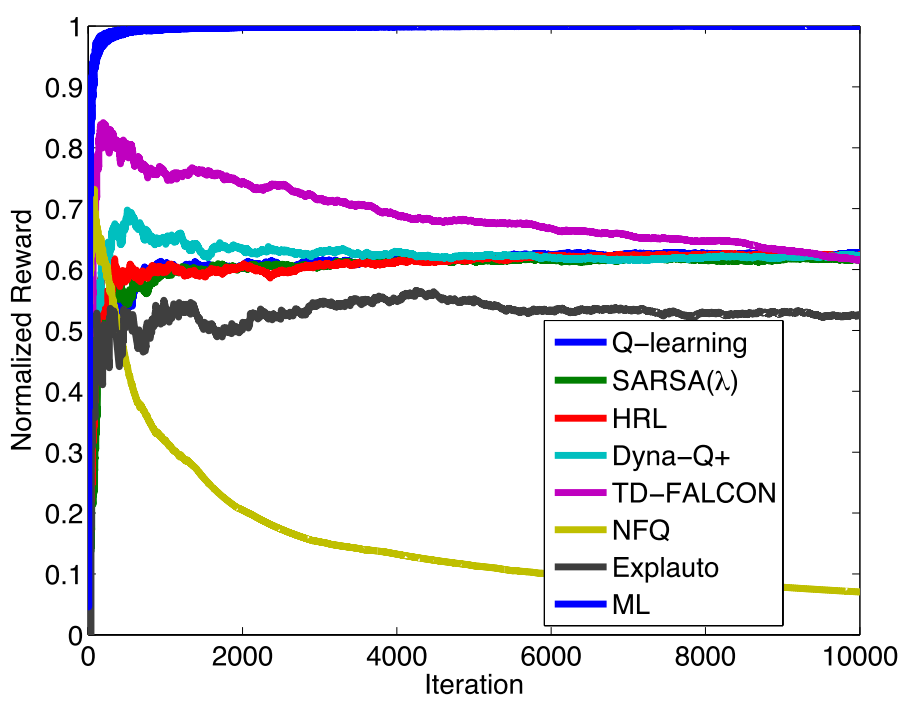
\includegraphics[width=0.55\linewidth]{rozdzial4/images/ml_vs_rl_blackbox_srate_1}
    \caption{Porównanie resultatów agenta ML z agentami RL dla $S_{rate}=1.0$. 
    Źródło: \cite{ml_vs_rl_comparative_study}.}
    \label{fig:ml_vs_rl_blackbox_srate1}
\end{figure}

Dla współczynnika $S_{rate}=1$ na początku większość agentów daje sobie radę 
porównywalnie tak samo. Sytuacja się zmienia już po około 500 iteracjach, 
gdzie wiele agentów przestaje sobie dawać radę w środowisku o coraz mniejszej
liczbie zasobów. Po około 2000 iteracjach większość agentów stabilizuje się
na tej samej wartości nagrody. Jedynym agentem, który daje sobie radę ze
zmnieniającym się otoczeniem jest agent z uczniem motywowanym. Wynika to
z najlepszego przystosowania do hierarchiczności świata tzn. zasobność 
surowców jest zależna od siebie hierarchicznie.  

Jeszcze bardziej zróżnicowane rezultaty i większe różnice pomiędzy agentem
z uczeniem motywowanym i agentem z uczeniem ze wzmocnieniem pojawiają
się dla współczynnika $S_{rate}=8.0$. Rezultaty widać na rysunku \ref{fig:ml_vs_rl_blackbox_srate8}.

\begin{figure}[h]
    \centering
    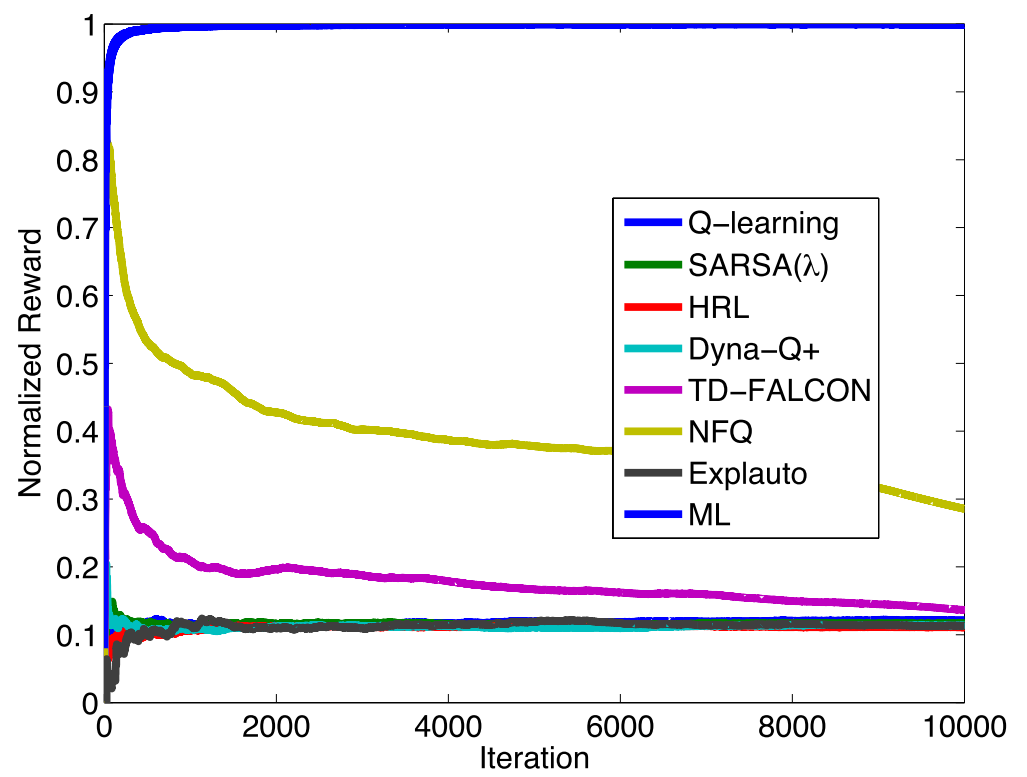
\includegraphics[width=0.6\linewidth]{rozdzial4/images/ml_vs_rl_blackbox_srate_8}
    \caption{Porównanie resultatów agenta ML z agentami RL dla $S_{rate}=8.0$. 
    Źródło: \cite{ml_vs_rl_comparative_study}.}
    \label{fig:ml_vs_rl_blackbox_srate8}
\end{figure}

Dla bardzo wrogiego środowiska, agent z uczeniem motywowanym daje sobie wciąż
radę, natomiast większość agentów z uczeniem ze wzmocnieniem, bardzo szybko 
stabilizuje się na niskiej wartości nagrody, ponieważ środowisko stało się
bardzo szybko wrogie poprzez niskie zasoby surowców. Agent z uczniem
motywowanym jest w stanie szybko stworzyć hierachię abstrokcyjnych bóli,
których obniżenie sprawia, że brakujące zasoby mogą zostać odbudowane.


\chapter{Środowisko symulacyjne}
\label{cha:rozdzial4}

Gdy projektowano pierwsze maszyny, które miały wykonywać konkretne zadania, opierano
się na dokładnych modelach matematycznych opisujących fizykę. Nie istniały narzędzia
do weryfikacji skuteczności działania danego urządzenia. Dopiero rozwój technologii
komputerowych i wzrost mocy obliczeniowej procesorów umożliwił bardzo szybką 
weryfikację stworzonych maszyn na komputerach, które w kilka sekund były w stanie 
sprawdzić poprawność obliczeń. Duże znaczenie symulacje zaczęły odgrywać kiedy
testowanie projektowanych maszyn mogło sprawiać zagrożenia dla ludzi czy samego
środowiska, w którym były testowane.

Ze względu na coraz niższą cenę sprzętu komputerowego i rozwojowi oprogramowania,
coraz więcej osób może w swoich domach uruchamiać modele wielu urządzeń bez ryzyka
uszkodzenia czegokolwiek i móc prowadzić swoje badania. W poniższej pracy konieczne
było zastosowanie takiego środowiska symulacyjnego, ponieważ testowane rozwiązania
są nowe i agenci uczenia motywowanego mogą czasem wykonywać czynności, które nie
były uwzględnione przez projektanta, zgodnie z tabelą \ref{tab:ml_vs_rl}.

W poniżej pracy uczenie motywowane będzie testowane na robocie mobilnym w środowisku
symulacyjnym Gazebo Sim \cite{gazebo_sim_website}.

\section{Symulator Gazebo}

Rozwój symulatora Gazebo rozpoczął się jesienią 2002 roku na Uniwersytecie 
Południowej Kalifornii. Oryginalnymi twórcami byli dr Andrew Howard i jego 
uczeń Nate Koenig. Koncepcja symulatora o wysokiej wierności wynikała z potrzeby 
symulacji robotów w środowiskach zewnętrznych w różnych warunkach. 
Jako komplementarny symulator do Stage, nazwa Gazebo została wybrana jako 
struktura najbliższa scenie zewnętrznej. Nazwa utknęła pomimo faktu, że 
większość użytkowników Gazebo symuluje środowisko wewnętrzne.

\begin{figure}[h]
    \centering
    
\includegraphics[width=0.3\linewidth]{rozdzial5/images/gazebo_logo}
    \caption{Logo Gazebo Sim. Źródło: \cite{gazebo_sim_website}.}
    \label{fig:gazebo_logo}
\end{figure}

Symulator ten ma zintegrowane silnik fizyki ODE (Open Dynamics Engine). Wykorzystuje
renderowanie korzystając z OpenGL. Dzięki temu możeliwe jest symulowanie wielu 
rodzajów sensorów:

\begin{itemize}
    \item ciśnieniomierz,
    \item wysokościomierz,
    \item kamera (RGB, głębi),
    \item czujnik kontaktu (dotyku),
    \item czujnik nacisku,
    \item GPS,
    \item lidar,
    \item skaner laserowy,
    \item IMU (ang. \textit{inertial measurement unit}),
    \item magnetometr,
    \item czujnik odległości,
    \item inne.
\end{itemize}

Tak duży zasób czujników umożliwia sprawdzanie na wiele sposobów jaki zestaw 
sensorów może być wykorzystany dla konkretnych celów oraz sprawia, że testowanie
nowych funkcjonalności bez ryzyka uszkodzenia robota czy środowiska. 

Graficzny interfejs umożliwia szybkie projektowanie nowych robotów czy elementów
środowiska. Wygląd głównego okna, w którym wykonywana jest większość pracy
podczas projektowania środowiska symulacyjnego pokazano na rysunku 
\ref{fig:gazebo_main_window}.

\begin{figure}[h]
    \centering
    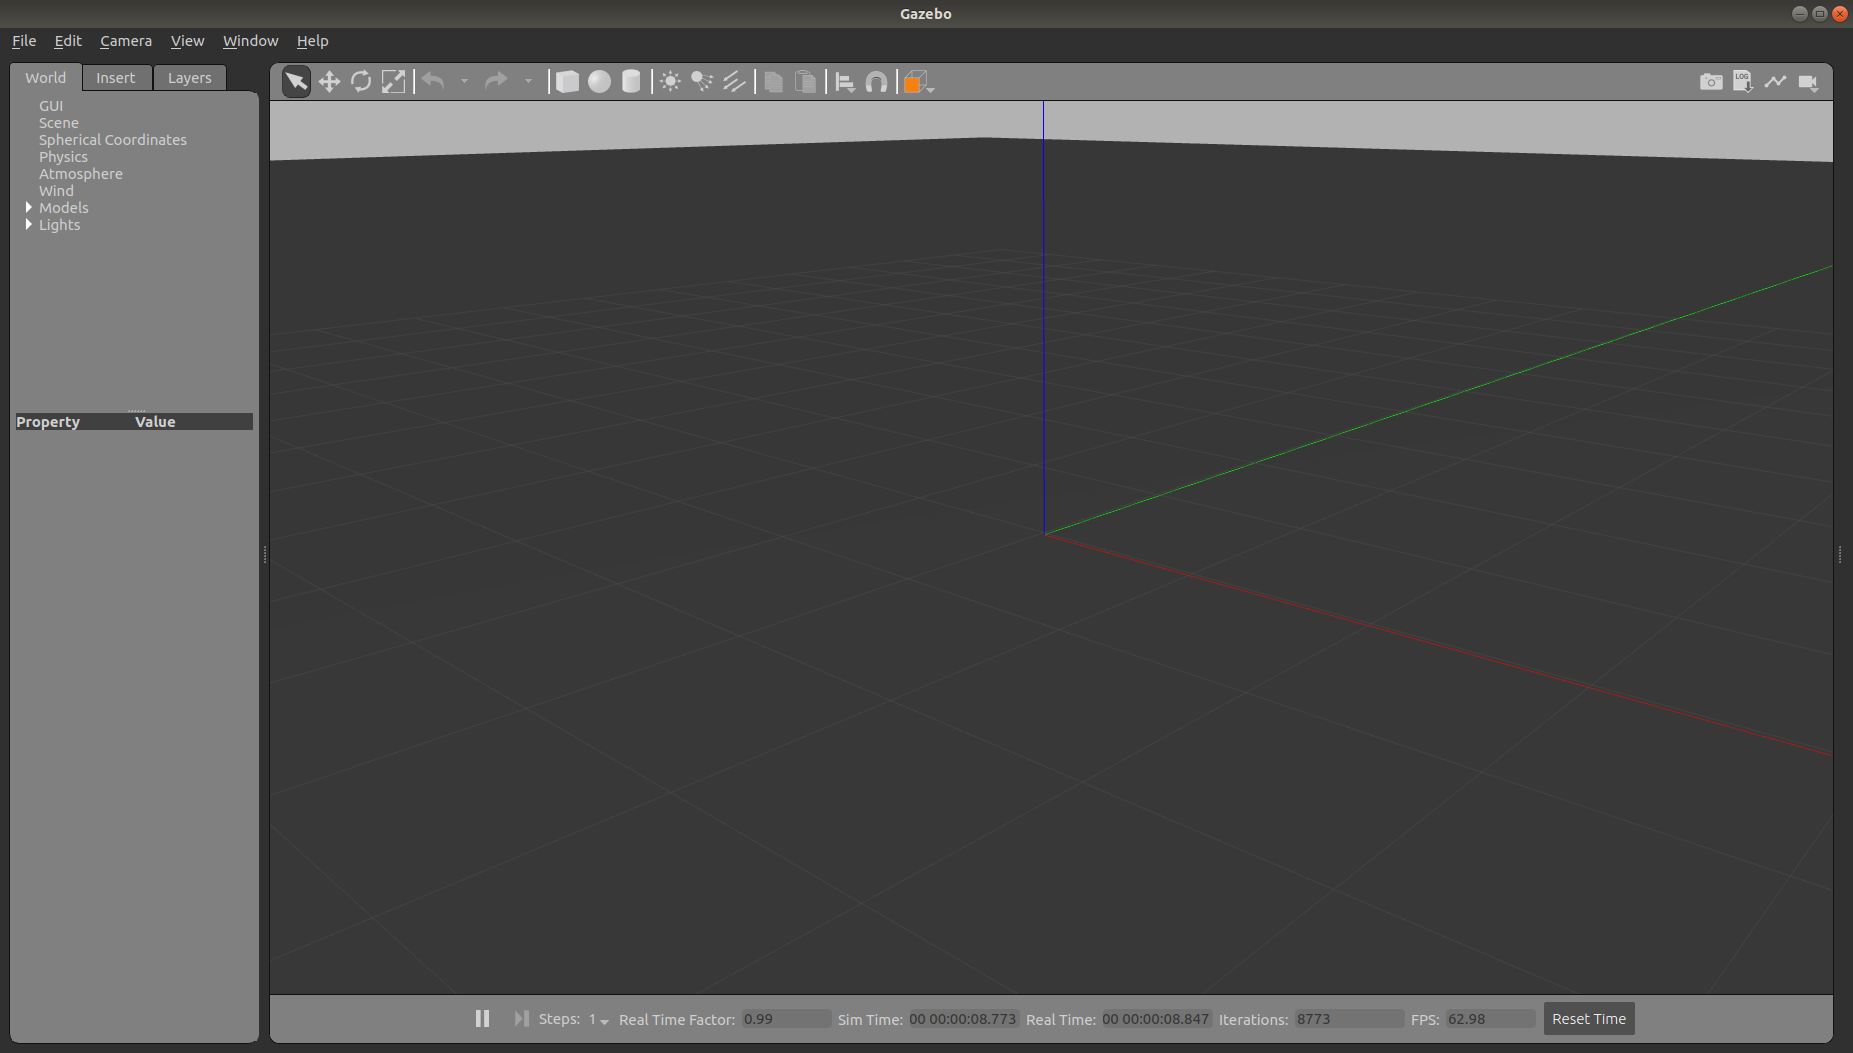
\includegraphics[width=0.7\linewidth]{rozdzial5/images/gazebo_main_window}
    \caption{Główne okna symulatora Gazebo. Źródło: opracowanie własne.}
    \label{fig:gazebo_main_window}
\end{figure}

Dodatkowowo w Gazebo oprócz silnika fizycznego ODE można skorzystać także z innych
bardzo popularnych silników fizyczny jak: Bullet. Dzięki rzeczywistemu renderowaniu
sceny w kamerach możliwe jest testowanie systemów wizyjnych. Takie na pewno
muszą być zastosowane dla agenta z uczeniem motywowanym, ponieważ to jeden
z podstawowych sensorów stosowanych przez człowieka na etapie poznawania nowego
środowiska.

Środowisko Gazebo Sim składa się z kilku elementów, które sprawiają, że możliwe
jest uruchomienie symulacji robota. Są to zgodnie z \cite{gazebo_components}.

\begin{itemize}
    \item \textbf{World files} -- pliki zawierające opis danego środowiska, 
    w którym robot ma działać, można w nich modyfikować parametry świata, 
    np. siłę grawitacji,
    \item \textbf{Model files} -- pliki w formacie SDF zawierające opisy 
    struktury robota,
    \item \textbf{Environment variables} -- zmienne środowiskowego, które 
    umożliwiają w prosty sposób uruchamiać Gazebo i ładować modele robotów 
    do symulacji,
    \item \textbf{Gazebo Server} -- główny program symulacji, który wykonuje 
    wszelkie obliczenia tj. liczenie kolizji, symulowanie czujników,
    \item \textbf{Graphical Client} -- umożliwia wyświetlanie wyników 
    obliczeń z serwera Gazebo,
    \item \textbf{Plugins} -- małe biblioteki, które umożliwiają w prosty 
    sposób wchodzić w interakcję w symulacją poprzez tworzenie własnych 
    sensorów czy wtyczek modyfikujących parametry świata z poziomu kodu.
\end{itemize}

Architektura całego systemu umożliwia proste projektowanie sensorów, robotów
czy całych środowisk do symulowania różnych scenariuszy środowiska jak 
parametry, np. siła grawitacji czy opory powietrza, jeżeli symulowane są roboty
latające jak drony. 

Gazebo używa rozproszonej architektury z rozdzielonymi bibliotekami do 
symulacji fizyki, renderowania sceny, interfejsu użytkownika, komunikacji i 
generowaniu sensorów. Dodatkowo w celu uruchomienia wszystkich możliwości 
symulatora, wcześniej wspomnianych: \textit{gzserver} do symulowania fizyki, 
renderowania i sensorów oraz \textit{gzclient}, który umożliwia wyświetlanie 
interfejsu użytkownika. Elementy architektury Gazebo przedstawiono na rysunku 
\ref{fig:gazebosystemarchitecture}:

\begin{figure}
	\centering
	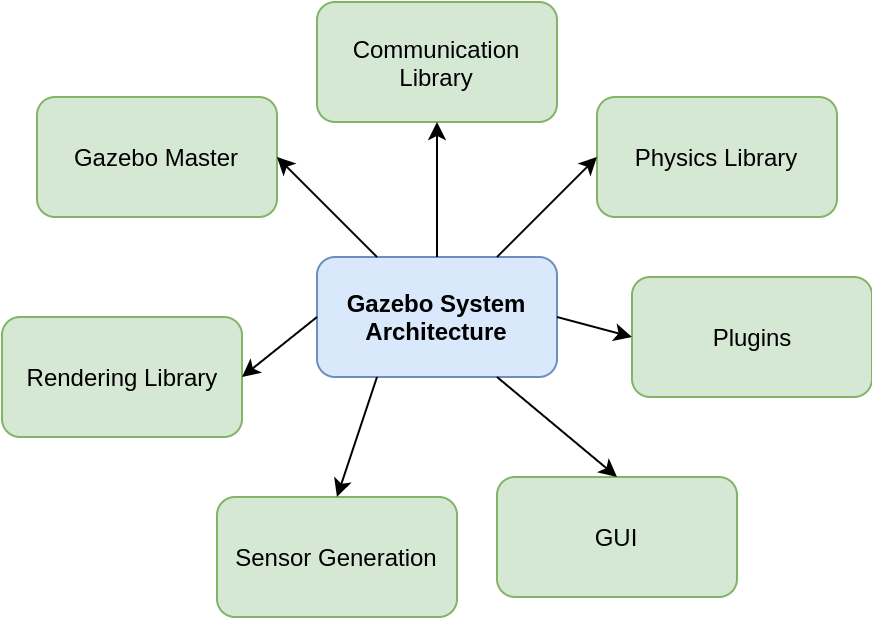
\includegraphics[width=0.7\linewidth]{rozdzial5/images/gazebo_system_architecture}
	\caption{Architektura systemu Gazebo. Źródło: opracowanie własne.}
	\label{fig:gazebosystemarchitecture}
\end{figure}


% itd.
% \appendix
% \include{dodatekA}
% \include{dodatekB}
% itd.

\printbibliography

\end{document}
